\chapter{PCA与异常检测}
\subsection{符号}
粗体大写字母表示的是矩阵,类似于${\bf X}$。粗体小写字母表示列向量,类似于${\bf x}$。希腊字母表示系数,类似于 $\lambda,\mu$。 $||{\bf X}||_F$ 表示矩阵 ${\bf X}$ 的F-范数,而 $||{\bf X}||_{1,1}$ 表示 ${\bf X}$ 的 $L_{1,1}$ 范数。也即 $||{\bf X}||_{1,1} = {\bf 1}|{\bf X}|{\bf 1}^T$。

数据集表示为一个 $n \times p$ 的数据矩阵 ${\bf D}$,其中每一个行向量表示一个$p$维的记录,而每一个列向量则是一个特征向量。${\bf A} = {\bf D}^T{\bf D}$是数据矩阵${\bf D}$的协方差矩阵。$Tr({\bf A})$ 表示矩阵 ${\bf A}$的迹。而$Card({\bf A})$ 表示矩阵${\bf A}$的势,即矩阵的非零元素个数。${\bf I}$是一个单位矩阵。$\mathbb{S}^p$ 是所有所有$p \times p$维矩阵即$\mathbb{R}^{p \times p}$的对称半正定矩阵构成的子集。

\subsection{PCA异常检测模型}
主成分分析(PCA)通常被用于进行特征压缩,即对于一个数据矩阵,他可以提取出体现了数据主要变化的一组特征,而这组特征是由数据原本的特征线性组合得到的。假设给定一个$p$维的数据集,即有$p$个特征,数据存在的$p$维欧氏空间命名为空间A,空间通过它的$p$个基向量来进行描述。虽然一个空间可以用无数组基向量来描述,但一般都通过最简洁的正交基进行描述,对于原始空间而言,最好的就是各个特征方向上的基向量,他们整体组成一个单位矩阵。而PCA所发掘的新的特征实际上是原始空间的一个子空间,在这一个子空间内,体现了数据的主要变化,即数据在这个子空间中总的方差最大,这个子空间在作为特征压缩应用时,我们称其为主要子空间。

使用PCA来进行异常检测的主要思路在于,对于整体而言主要变化同时体现的也是主流的变化,即大多数的数据点都能够很好的用降维的特征来进行描述,对这些个体而言,它们在PCA得到的主要子空间内的投影向量与自身基本相符。但同时还存在一些数据点,如果用降维得到的特征来进行描述将会丢失很多信息,即它们在PCA得到的主要子空间内的投影向量与自身差异较大。

举例而言,用太阳系八大行星加上冥王星的三维运行轨迹点作为分析数据集,我们将会发现,数据的主要变化都在黄道平面上,因此,实际上我们可以只用黄道平面上的坐标就足够描述行星运动。八大行星的运动都能很好的用黄道平面坐标描述,但是冥王星在黄道平面上的投影向量与自身实际位置向量常常会有很大的偏差,因此,我们可以判别冥王星的运动不符合主流。而事实上,其运动不符合主流也是冥王星被排除出太阳系大行星行列的主要原因之一。

之前提到,数据的主要变化体现了数据的主流变化,但其实这个判断在一些情况下并不准确。因为有的时候非主流的变化可能会对整体变化造成非常大的影响,这在实际生活中并不鲜见。在统计分析中,摒除掉非主流样例对把握主流特征的干扰被称为鲁棒统计分析,PCA同样也有一部分分支为鲁棒PCA分析(Robust PCA),并且这一类分析也被运用到了异常检测当中。我们的工作没有讨论这一部分的延伸,但可以通过一些初步的处理来去除掉异常数据点的对主流规律的干扰,例如将一些数值明显超出正常范畴的数据点不纳入到PCA得到主要子空间的分析数据内。

另外,PCA异常检测得到的是数据中的非主流数据点,在实际生活中,非主流数据点未必是非正常数据点即异常数据点,主流并不是正常的同义词。但在非监督的统计分析当中,也只能检测得到非主流的信息,而大多数情况下,非主流和异常是存在大量重合的。

在异常检测任务中,我们将主要子空间称为正常子空间,而与之互补的子空间称为异常子空间。

PCA分析得到的是一系列构成新特征的系数向量以及数据依据系数向量所构成的${\bf 主成分}$。第一个主成分是数据集下,能够获取最大方差的特征方向上的投影值。随后的主成分则是与之前的主成分线性无关条件下所能获取的最大方差特征方向上的投影值。前$k$个主成分以及相应的系数向量构成了主要子空间,即正常子空间。其中系数向量即为空间的正交基。而剩余的主成分和系数向量则构成了异常子空间。

如前所述,判断一个数据点是否为异常的依据是该数据点向量与其在正常子空间下的投影向量的偏差\cite{PCA-Sensitivity}。用数学符号来表达即为:

定义 ${\bf V}_1=({\bf v}_1,\cdots,{\bf v}_k)$ 为靠前的$k$个主成分所处的正常子空间,${\bf v}_1,\cdots,{\bf v}_k$ 是各个主成分所对应的系数向量,系数向量互相垂直。而${\bf V}_2=({\bf v}_{k+1}, \cdots,$ ${\bf v}_p)$ 则是剩余的 $p-k$ 个主成分所处的异常子空间,同样是通过主成分所对应的系数向量 ${\bf v}_{k+1},\cdots,{\bf v}_p$ 作为基向量来构建该子空间。对于一个 $p$ 维的数据点 $y$,其自身与其在正常子空间下的投影向量的偏差 $\hat{{\bf y}}$ 可以表示为:

\begin{equation}
\hat{{\bf y}} = {\bf y}-{\bf V}_1{\bf V}_1^T{\bf y}.
\end{equation}

${\bf \hat{y}}$的平方长度被称为SPE(squared prediction error),即通过PCA来预测还原数据的误差。SPE是PCA模型用来判定数据点 ${\bf y}$ 是否异常的指标。SPE越大,则该数据点越可能是一个异常。实际使用中,会设置一个阈值来判断是否异常,阈值的大小由使用者从准确率以及回归率等方面进行权衡。

\subsection{异常解释}

而如何理解判定其为异常的依据,即数据点 ${\bf y}$ 哪些方面的表现使得他的与正常子空间下投影的偏差过大,即PCA模型异常检测的异常解释问题。虽然偏差向量 $\hat{{\bf y}}$ 的长度是检测异常的主要依据,但用 $\hat{{\bf y}}$ 向量本身的各个维度上的值来解释是没有意义的。因为这些维度上的值并不该数据点 ${\bf y}$ 原本特征维度上的数值有直接的对应关系\cite{PCA-Sensitivity},也就是说,这些值的来源很难解释。

正常子空间${\bf V}_1$下向量与投影的偏差$\hat{{\bf y}}$其实就是向量在正常空间的补空间即异常子空间 ${\bf V}_2$ 上的投影,即有:

\begin{equation}
\label{equation:yHat}
\begin{split}
\hat{\bf{y}} &= {\bf y}-{\bf V}_1{\bf V}_1^T{\bf y} \\
 & = {\bf V}_2{\bf V}_2^T{\bf y}.
\end{split}
\end{equation}

我们设定异常子空间 ${\bf V}_2=({\bf v}_{k+1}, \cdots, {\bf v}_p)$,其中 ${\bf v}_{k+1},\cdots,{\bf v}_p$ 是一组互相垂直的系数向量,由他们作为正交基来表示异常子空间。依据\ref{equation:yHat},可以得到SPE为:


\begin{equation}
\label{equation:SPE}
\begin{split}
SPE &= \hat{{\bf y}}^T\hat{{\bf y}} = {\bf y}^T{\bf V}_2 {\bf V}_2^T {\bf V}_2 {\bf V}_2^T {\bf y}\\
       & = ({\bf y}^T{\bf V}_2)({\bf V}_2^T {\bf V}_2)({\bf V}_2^T {\bf y})\\
       & = ({\bf V}_2^T {\bf y})^T({\bf V}_2^T {\bf y})\\
       & = \sum_{i=k+1}^{p}({\bf v}_i^T {\bf y})^2.
\end{split}
\end{equation}


\begin{figure}
	\centering
	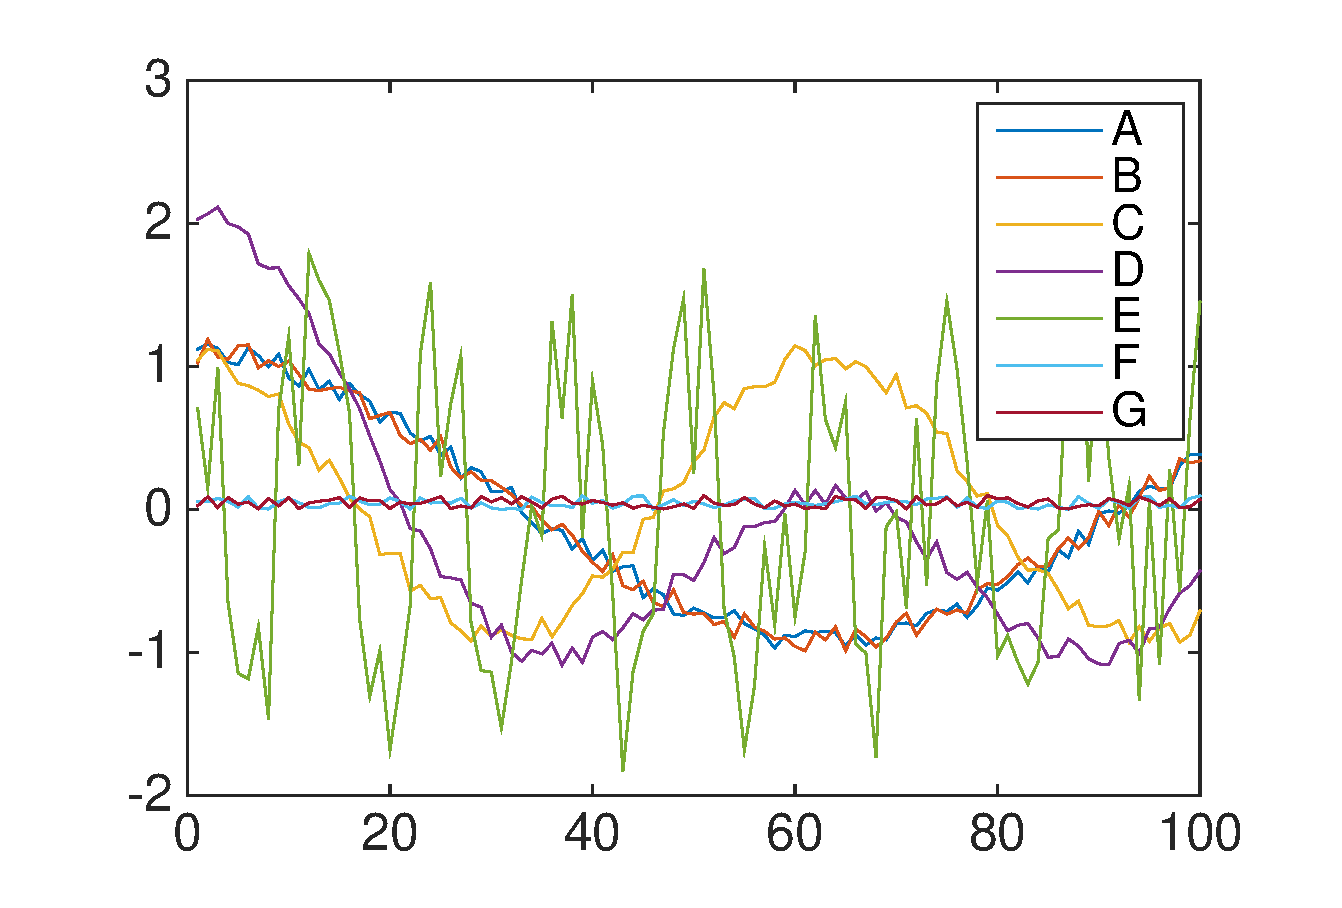
\includegraphics[width=80mm]{figure/lines/synthesized_data}
	\label{fig:synthesized_data}
	\caption{合成数据中的正常样例}
\end{figure}


\begin{figure}
\begin{minipage}{0.48\textwidth}
\centering
\includegraphics[height=50mm]{figure/new/Synthetic-Components-PCA}
\label{fig:pcs:PCA}
\caption{PCA}
\end{minipage}\hfill
\begin{minipage}{0.48\textwidth}
\centering
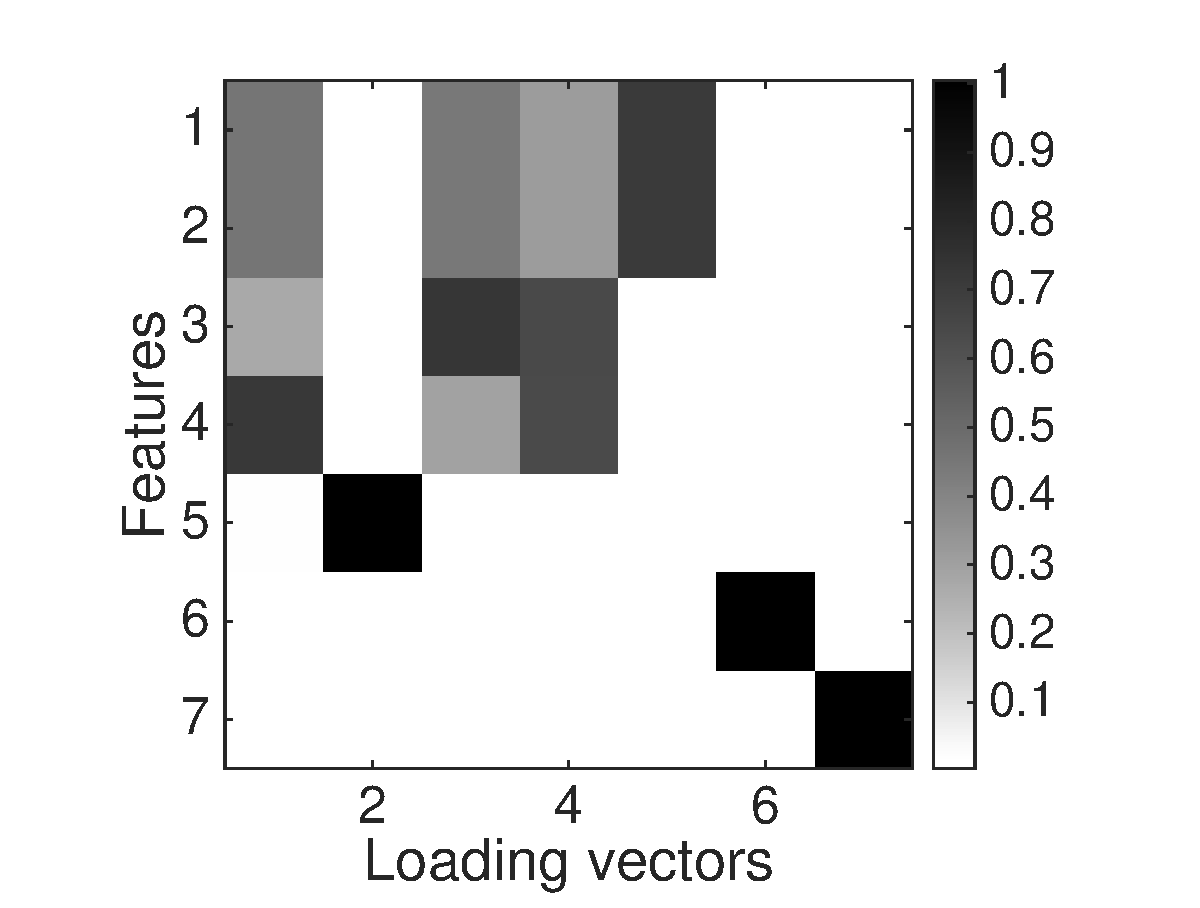
\includegraphics[height=50mm]{figure/new/Synthetic-Components-ASPCA-F}
\label{fig:pcs:ASPCA}
\caption{ASPCA}
\end{minipage}
\caption{Synthetic data and loading matrices obtained by PCA and ASPCA}
\label{fig:mappingmatrix}
\end{figure}

由\ref{equation:SPE}可知,SPE的计算并不需要通过计算两次空间投影后的向量,只需要计算一次空间变换后的长度即可。即SPE等于 ${\bf y}$ 在系数向量上的标量投影的平方和。因此我们可以认为,计算SPE的加和等式中,对于总和超过阈值有着突出贡献的加数对于该数据点被判别为异常点有很关键的作用。每个这样的加数,分别是数据点 ${\bf y}$ 在系数向量上投影的平方和,同时也是数据各个特征依据系数向量给予的组合方式之后所求出的值的平方。

因此,PCA判别异常除了数据无法被正常子空间所完全描述以外,还有另一种解释方法。即,数据点的各个特征按照一系列指定的参数关系相加之后所产生的一系列数值在正常情况下都是很小的,而在异常情况下,这一系列数值的平方和相加超过判定的阈值。也就是说,异常产生可以被视为是一些数据点违背了正常情况下数据所遵守的一些线性规律。

同样用之前关于行星轨迹的例子来解释,八大行星所遵循的是在与黄道平面垂直的$z$轴的值基本为零,而冥王星则常常打破这个约束。

但是在更普遍的场景下,所提到的这些PCA所挖掘的线性规律,也即异常主成分的系数向量,也即异常子空间的基向量是非常复杂的,涉及到很多原本的特征,远远不想行星轨迹那样只涉及到一个$z$轴上的运动值。因此,异常点仍然无法解释。为了使他们变得清晰简洁,我们希望他们能够具有稀疏的性质。

因此,我们提出了我们自己的改进模型。新的模型希望获取异常子空间的一组新的基向量,这些基向量同时具有正交稀疏的性质。这种基向量所构造的异常子空间将能够同时完成异常检测和异常诊断任务。正交性确保等式~\ref{equation:SPE}成立,而稀疏性提供保证了每一条线性关系的简明易读。我们将该模型称为异常子空间稀疏PCA即Abnormal Subspace Sparse PCA(ASPCA)。

对于一个异常而言,他对线性关系的违背超过了阈值,这里涉及到的线性关系可能只是少数几条,但也可能出现涉及很多的情况。我们判断是某条线性关系否涉及的依据是对该关系的违背情况与阈值的相对大小。理论上,可能会出现很多关系的违背影响力都很大的情况,也可能出现大量关系的违背情况都很微小,但相加的总和却超过了阈值的情况。但实际使用中发现,大多数异常都还是在部分特征上有所体现,因此较少出现以上所陈述的两种情况。而如何在模型中考虑这种问题,即在关于异常子空间基向量的稀疏性与正交性约束之外再加上一条,异常在基向量的投影的稀疏性,也在我们的后续工作中继续研究。 

我们构造了一个由500个正例与15个反例构成的数据集来进行演示。其中最前面的100歌正例如图~\ref{fig:synthesized_data})所示。每一个数据点有七个特征,分别命名为$A$ 到 $G$,且正常的数据通过4种模式进行生成,即$A \approx B$,$D \approx C + A$,$F \approx 0$,$G \approx 0$。反例则有三种类型,分别通过打破前三种模式进行生成。通过PCA得到的主成分参数矩阵如图~\ref{fig:pcs:PCA}所示,其中PCA得到的靠后的四个主成分即异常主成分,很难进行解读。当我们通过我们之后将会介绍的算法,根据我们要求稀疏性和正交性的ASPCA模型所得到的主成分参数矩阵如图~\ref{fig:pcs:ASPCA}所示,这样得到的靠后的四个异常主成分的系数向量,将可以很好的在异常检测的同时完成异常诊断任务。

ASPCA模型将异常的解释分成两个步骤,首先,我们分析样本在哪些异常基向量上的投影,即对线性关系的违背,对于SPE有很高的贡献,这依据的是等式~\ref{equation:SPE}。然后,阐释这些不同的线性关系。

\begin{figure}
	\centering
	\includegraphics[height=30mm]{figure/new/Synthetic-Components-JSPCA}
\caption{Loading matrix obtained by JSPCA}
\label{fig:loading matrix:synthetic}
\end{figure}

相关工作中所提到的 Jiang 等人所做的工作\cite{jiang2013family},即联合稀疏PCA(JSPCA)同样是通过获取异常子空间的稀疏表达来进行异常分析。但他们的主要思路是从整体上用较少的特征来近似表达异常子空间,这种方式下,所有的系数向量都是由相同的少数几个特征来进行表达如图\ref{fig:loading matrix:synthetic}。尽管JSPCA获取到了与异常相关联的特征维度,但是他有两个主要限制。其一,JSPCA所识别的特征是从数据集中所有异常角度进行考虑的,即他所捕捉的是所有异常所体现的主要特征。当异常存在不同类别时,不同种类的异常应当有不同的表现,这在网络入侵检测,系统异常检测等场景下也是很普遍的现象。而对于这样的情况,JSPCA无法给不同种类的异常不同的解释。对于一个无监督异常检测任务,JSPCA显然不能假定异常只有一种类别内。其二,JSPCA识别了异常的主要相关特征,但并没有阐释这样的特征是如何导致记录点被判定为异常,即没有给出直接的依据。

\subsection{ASPCA模型}

以上,我们提出了一个新的异常检测解释模型ASPCA,以下我们将介绍ASPCA的两种求解方式。

首先,对于正常空间稀疏PCA问题的求解,普遍有两种思路,其一是整体解法,其二是逐步解法\cite{SPCA-SDP}。

整体解法的思路是构造一组子空间的稀疏基向量,在这组基向量上,数据将能够最好的进行还原,即原始数据与投影后的数据偏差最小。如果按照这样的思路进行计算,ASPCA模型需要的是投影后本身最小的一个子空间,因为异常子空间本身就是原始数据与正常子空间投影的偏差。但是,这种解法并没有约束子空间的各个基向量具有正交性质,而在添加了正交约束后,原本的优化方法不再适用。因此我们选择了另一种思路,即逐步解法。

逐步解法的思路是每次只计算求解一个稀疏基向量,该基向量具有稀疏的性质,并且数据在该基向量上有最大的方差。随后将已经被求解出的基向量所覆盖的变化从数据中剔除出去,再用修改后的数据求出第二个基向量,同样的步骤继续下去直到所有基向量都被求解出来。如果按照这样的思路,ASPCA模型同样需要考虑基向量正交的问题,而一般所用的修改数据的方式来逐个求解基向量的方式无法保证该约束,因此我们不采用修改数据的方式,而是直接添加正交性要求,即:当前求解出的基向量必须与之前已经求解的基向量正交。并且,我们可以通过一些条件的放松,利用半正定规划求解该优化问题。

总之,我们通过在逐步解法添加正交性约束,去除掉修改数据的步骤,实现了我们ASPCA模型的第一个解法,我们将其称之为${\bf 前向ASPCA}$ 即 ASPCA-F。

给定数据的协方差矩阵 ${\bf A}$ ,以及对稀疏性的要求参数 $k$,对于每一个基向量${{\bf v}_i},i = 1,...,p$的计算,ASPCA-F所要优化的目标函数为:

\begin{equation}
\label{equation:typical_MSPCA-F}
\begin{split}
& \argmax_{{\bf v}_i}\ {\bf v}_i^T{\bf A}{\bf v}_i\\
 s.t. & \ {\bf v}_i^T{\bf v}_i=1,\ Card({\bf v}_i)\leq k, \\
 &\ {\bf v}_i^T{\bf v}_j=0\ \forall 1\leq j<i. 
 \end{split}
\end{equation}

ASPCA-F所获取的$p$条向量中,靠前先获取的向量构成正常子空间,而靠后的向量构成异常子空间。

ASPCA-F的主要问题在于,它优先获取了正常子空间的稀疏表示,但这并不是我们所需要的。而如果对于ASPCA-F先求解出来的向量不给予稀疏性的限制,而只对后获取的用来构建异常子空间的向量加上稀疏性限制,由于异常子空间需要与正常子空间正交,因此会受到正常子空间影响。总之,求解异常子空间之前需要先求解正常子空间是导致ASPCA-F不令人满意的主要原因。

因此,我们提出了另一种解法,即直接求解异常子空间,即先求解方差最小的主成分,将之前的整个求解过程逆转过来。我们将这种解法称为${\bf 后向ASPCA}$即$ASPCA-B$。这种求解方式下,优先保证异常子空间的稀疏性。由于PCA求解原本就可以从最小主成分开始计算,正如\ref{prop:reverse}所证,因此ASPCA-B从后往前计算也是合理的。其中PCA所求解的主成分所对应的向量就是数据协方差矩阵的特征向量,而构成正常子空间的基向量就是最大的若干个特征向量,异常子空间则是较小的特征向量。因此,我们证明的是对于协方差矩阵${\bf A}$,可以先求出最小的若干特征值所对应的特征向量,再求出较大的特征值与特征向量。

\begin{proposition}
\label{prop:reverse}
给定协方差矩阵 ${\bf A} = {\bf D}^T{\bf D}$,如果我们已经提取了对应于$n-k-1$个最小特征值的正交特征向量 ${\bf v}_{k+1},{\bf v}_{k+2},....,{\bf v}_n$,剩余的没有被提取的特征值从大到小为 $\lambda_1 \geq \lambda_2 \geq ... \geq \lambda_k$,对应的特征向量为 ${\bf v}_1, {\bf v}_2,....,{\bf v}_k$,所有特征向量相互垂直 ,则表达式\ref{equation:proposition:init} 的解即为特征值$\lambda_k$所对应的特征向量.
\begin{equation}
\begin{split}
 & \argmin_{{\bf v}}\ {\bf v}^T{\bf A}{\bf v}\\
 s.t. & {\bf v}^T{\bf v} =1,\ {\bf v}^T{\bf v}_i=0\ \forall k<i\leq n
\end{split}
\label{equation:proposition:init}
\end{equation}
\end{proposition}
\begin{proof}
将 ${\bf v}$ 投影到 $({\bf v}_1,...,{\bf v}_n)$,可以得到 ${\bf v} = \sum_{i=1}^{n} \alpha_i {\bf v}_i$,其中 $\alpha_i = {\bf v}^T{\bf v}_i$。又因为有限制条件 ${\bf v}^T{\bf v}_i=0\ \forall k<i\leq n$ 因此可得 $\alpha_i = 0\  \forall k<i\leq n$,即可得${\bf v} = \sum_{i=1}^{k} \alpha_i {\bf v}_i$。

优化目标${\bf v}^T{\bf A}{\bf v}$ 可以展开为:

\begin{equation*}
\begin{split}
 & {\bf v}^T{\bf A}{\bf v}\\
 =& (\sum_{i=1}^{k} \alpha_i {\bf v_i})(\sum_{i=1}^{k} \alpha_i {\bf A}{\bf v}_i)\\
 =& (\sum_{i=1}^{k} \alpha_i {\bf v}_i)(\sum_{i=1}^{k} \alpha_i \lambda_i  {\bf v}_i)\\
 =& \sum_{i=1}^{k} \alpha_i^2 \lambda_i {\bf v}_i^T {\bf v}_i + \sum_{i=1}^{k} \sum_{j=1,j \neq i}^{k} \alpha_i \alpha_j \lambda_j {\bf v}_i^T {\bf v}_j
\end{split}
\end{equation*}

由于${\bf v}_i^T{\bf v}_j=0, i \neq j$,因此可得 $\sum_{i=1}^{k} \sum_{j=1,j \neq i}^{k} \alpha_i \alpha_j \lambda_j {\bf v}_i^T {\bf v}_j = 0$。由此得到:

\begin{equation}
\label{equa:vAv}
{\bf v}^T{\bf A}{\bf v} = \sum_{i=1}^{k} \alpha_i^2 \lambda_i
\end{equation}

由于 $\lambda_i \geq \lambda_k \ \forall i\leq k$,因此可得:

\begin{equation*}
\begin{split}
	{\bf v}^T{\bf A}{\bf v} = \sum_{i=1}^{k} \alpha_i^2 \lambda_i \geq \sum_{i=1}^{k} \alpha_i^2 \lambda_k = \lambda_k  \sum_{i=1}^{k} \alpha_i^2
\end{split}
\end{equation*}

由于${\bf v}^T{\bf v} = \sum_{i=1}^{k} \alpha_i^2 = 1$,可以得到:

\begin{equation}
\label{equa:geq}
	{\bf v}^T{\bf A}{\bf v} \geq \lambda_k 
\end{equation}

由于${\bf v}_k$ 符合${\bf v}$所需要满足的约束,因此是优化问题的待选解之一,但将${\bf v}_k$代入后的值一定不会优于最优解。因此可得:

\begin{equation}
\label{equa:leq}
\min_{\bf v}{{\bf v}^T{\bf A}{\bf v}} \leq {\bf v}_k^T{\bf A}{\bf v}_k = \lambda_k
\end{equation}

结合两个方向的不等式,即表达式~\ref{equa:geq}与表达式~\ref{equa:leq}可以得到:

\begin{equation}
\label{equa:equalK}
\min_{\bf v}{{\bf v}^T{\bf A}{\bf v}} = \lambda_k
\end{equation}

假设最优值为 $\hat{{\bf v}} = \sum_{i=1}^{k} \hat{\alpha}_i {\bf v}_i$,由表达式~\ref{equa:vAv} 可知有$\hat{{\bf v}}^T{\bf A}\hat{{\bf v}} = \sum_{i=1}^{k} \hat{\alpha}_i^2 \lambda_i$ ,又通过表达式~\ref{equa:equalK} 可知有$\hat{{\bf v}}^T{\bf A}\hat{{\bf v}} = \lambda_k$,因此可得:
\begin{equation*}
\begin{split}
\lambda_k - \sum_{i=1}^{k} \hat{\alpha}_i^2 \lambda_i = \sum_{i=1}^{k} \hat{\alpha}_i^2 (\lambda_k - \lambda_i) = 0 
\end{split}
\end{equation*}
由于 $\lambda_k - \lambda_i\leq 0,\forall i<k$,所以 $\hat{\alpha}_i^2 (\lambda_k - \lambda_i) $ 每一项都大于等于零,而求和是零,因此每一项都为零。因此可得 $\hat{\alpha}_i \neq 0$ 的必要条件是 $\lambda_i = \lambda_k$。因此可知,$\hat{{\bf v}}$ 是特征值为 $\lambda_k$  所对应的特征向量的线性组合。因而 $\hat{{\bf v}}$ 自己也是一个特征向量,对应的特征值为$\lambda_k$。
\end{proof}

显然,我们的证明对于 $k=n$ 也是成立的。 通过表达式~\ref{equation:proposition:init},我们可以从小到大的逐个计算特征值所对应的特征向量。在表达式~\ref{equation:proposition:init} 的基础上加上稀疏性限制则形成了ASPCA-B的优化目标。

给定协方差矩阵 ${\bf A}$ 以及稀疏性限制参数 $k$, 对于每一个基向量 ${\bf v_i},\ i = 1,...,d$ 的计算, ASPCA-B的优化目标函数为:
\begin{equation}
\label{equation:typical_MSPCA-B}
\begin{split}
 &\argmin_{{\bf v}_i}\ {\bf v}_i^T{\bf A}{\bf v}_i\\
s.t. &\ {\bf v}_i^T{\bf v}_i=1,  Card({\bf v}_i)\leq k. \\
& {\bf v}_i^T{\bf v}_j=0\ \forall 1\leq j<i,
 \end{split}
\end{equation}

ASPCA-B所提取的前 $d$ 个向量 $\bf{v}_1...\bf{v}_d$ 构成了我们所需要的异常子空间 ${\bf S}_a$,而剩余的补空间则是正常子空间。我们直接使用数据点在异常子空间下的投影来完成异常的检测与解释。
